\documentclass[serif,mathserif, 12pt]{beamer}
\usepackage{etex}
\usepackage{amsmath, amsfonts, epsfig, xspace}
\usepackage{algorithm,algorithmic}
\usepackage{pstricks,pst-node}
\usepackage{multimedia}
\usepackage[normal,tight,center]{subfigure}
\setlength{\subfigcapskip}{-.5em}
\usepackage{tkz-euclide}
\usetkzobj{all}
\usepackage{beamerthemesplit}
\usetheme{lankton-keynote}
\usepackage{graphicx,color}
% remove caption of figure
\usepackage[labelformat=empty]{caption}

\usepackage[none]{hyphenat} % hyphenation is ugly in slides
\usepackage{parskip}

\usepackage{relsize} % \smaller to change size

\usepackage{tikz}
\usetikzlibrary{calc}

\usetikzlibrary{arrows}

\newcommand{\TikzDraw}[2][]{
  \begin{tikzpicture}[overlay, remember picture, shift={(current page.center)}, #1]
    #2
  \end{tikzpicture}
}

\newcommand{\gridlines}{
  \TikzDraw{
    \draw[help lines,xstep=.2,ystep=.2,red!20] (current page.south west) grid (current page.north east);
    \draw[help lines,xstep=1,ystep=1,red] (current page.south west) grid (current page.north east);
    \foreach \x in {-15,-14,...,15} {
      \node [anchor=north, red] at (\x,0) {\tiny \x};
      \node [anchor=east,red] at (0,\x) {\tiny \x};
    }
  }
}

\newcommand{\DrawOnImg}[3][]
{
  \begin{tikzpicture}
    \node[anchor=south west,inner sep=0] (image) at (0,0){
      #2
    };
    \begin{scope}[x={(image.south east)},y={(image.north west)}]
      \ifthenelse{\equal{#1}{grid}}
                 {\draw[color=blue, style=dashed] (0,0) grid[xstep=.1, ystep=.1] (1.0001,1.0001);}
                 {}
                 #3
    \end{scope}
  \end{tikzpicture}
}

\usetikzlibrary{matrix}

\newcommand{\BOLD}[1]{\mathbf{#1}}
\newcommand{\BOLDG}[1]{\boldsymbol{#1}}
\newcommand{\PDIF}[2]{\frac{\partial #1}{\partial #2}}
\newcommand{\TODO}[1]{\textcolor{red}{#1}}
\newcommand{\TODOB}[1]{\textcolor{blue}{#1}}
\newcommand{\TODOG}[1]{\textcolor{green!50!black}{#1}}
\newcommand{\argmin}{\operatornamewithlimits{arg\min}}
\DeclareMathOperator{\tr}{tr}
\DeclareMathOperator{\cond}{cond}
\DeclareMathOperator{\ST}{s.t.}
\DeclareMathOperator{\diag}{diag}
\DeclareMathOperator{\Div}{div}

\title[\hspace{2em}\insertframenumber/\inserttotalframenumber]{Spectral Affine-Kernel Embeddings}
\date{May 8th, 2017}

\author{Max Budninskiy, Beibei Liu,\\ Yiying Tong, Mathieu Desbrun}

\begin{document}

\maketitle

\begin{frame}
  \frametitle{Embedding}
  \begin{itemize}
  \item High dimensional data often relies on or near a much
    lower dimensional, curved manifold.
  \end{itemize}
\end{frame}

\begin{frame}
  \frametitle{Embedding}
  \begin{itemize}
  \item Mapping high dimensional data into lower dimensional space with
    low distortion.
    \begin{itemize}
    \item[-] Surface parameterization
    \item[-] Mesh deformation
    \item[-] Feature extraction
    \item[-] ...
    \end{itemize}
  \end{itemize}
\end{frame}

\begin{frame}
  \frametitle{Linear approach}
  \begin{itemize}
  \item PCA, SVD
    \begin{itemize}
    \item \textcolor{red}{Pros: simple and robust.}
    \item \textcolor{green!50!black}{Cons: requiring data is close to forming a linear subspace.}
    \end{itemize}
  \end{itemize}
\end{frame}

\begin{frame}
  \frametitle{Nonlinear approach}
  \begin{itemize}
  \item Global approach: Isomap
    \begin{itemize}
    \item[-] Determine the neighbors of each point
    \item[-] Construct a neighborhood graph
    \item[-] Compute shortest path between two nodes
    \item[-] Compute lower-dimensional embedding
      \begin{itemize}
      \item[*] Multidimensional scaling
        \begin{equation*}
          cost = \sum_{i, j} (\|y_i-y_j\|-\|x_i-x_j\|)^2
        \end{equation*}
      \end{itemize}
    \end{itemize}
  \end{itemize}
\end{frame}

\begin{frame}
  \frametitle{Nonlinear approach}
  \begin{itemize}
  \item Disadvantages
    \begin{itemize}
    \item Inefficient computation of pairwise geodesic distance
    \item Geodesic distance computation is not accurate enough
    \item Solve for embedding is computational demanding
      \begin{itemize}
      \item[-] SVD of $n\times n$ dense matrix
      \end{itemize}
    \end{itemize}
  \end{itemize}
\end{frame}

\begin{frame}
  \frametitle{Nonlinear approach}
  \begin{itemize}
  \item Local approach
    \begin{itemize}
    \item[-] Locally Linear Embeddings, Laplacian Eigenmaps, Local Tangent Space Alignment
      \begin{figure}
        \centering
        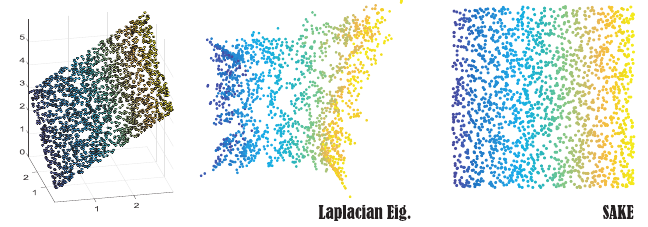
\includegraphics[width=0.8\textwidth]{img/affine_precision}
      \end{figure}
    \end{itemize}
  \end{itemize}
\end{frame}

\begin{frame}
  \frametitle{Rationale}
  \begin{itemize}
  \item Achieve as-isometric-as-possible embedding by \TODO{preserving relative position locally}
    between points.
  \end{itemize}
\end{frame}

\begin{frame}
  \frametitle{Input \& Ouput}
  \begin{itemize}
  \item Input
    \begin{itemize}
    \item[-] Point set $\{x_i\}_{i=1...n} \in R^D$ sampled from a connected $d$-manifold.
    \end{itemize}
  \item Output
    \begin{itemize}
    \item[-] Most isometric embedding $\{z_i\}_{i=1\dots n} \in R^d$.
    \end{itemize}
  \end{itemize}
\end{frame}

\begin{frame}
  \frametitle{Pipeline}
  \begin{itemize}
  \item Construct a proximity graph $G$
  \item Compute for each $x_i$ an isomap of its neighborhood
  \item From each of resulting embedding, assemble a local linear
    operator $L_i$.
  \item Assemble a global quadratic form $Q$ from $L_i$, and
    find the final embedding.
  \end{itemize}
\end{frame}

\begin{frame}
  \frametitle{Proximity graph}
  \begin{itemize}
  \item Traditional approach: connect K-nearest neighbors
  \item Small $k$ to linking points and construct graph
    \begin{itemize}
    \item[-] Better approximation of geodesic distance
    \end{itemize}
  \item Larger $K$ to define the neighborhood
    \begin{itemize}
    \item[-] Robust to noise
    \end{itemize}
  \end{itemize}
\end{frame}

\begin{frame}
  \frametitle{Proximity graph}
  \TikzDraw {
    \visible<1> {
      \node at (0, 0) {
        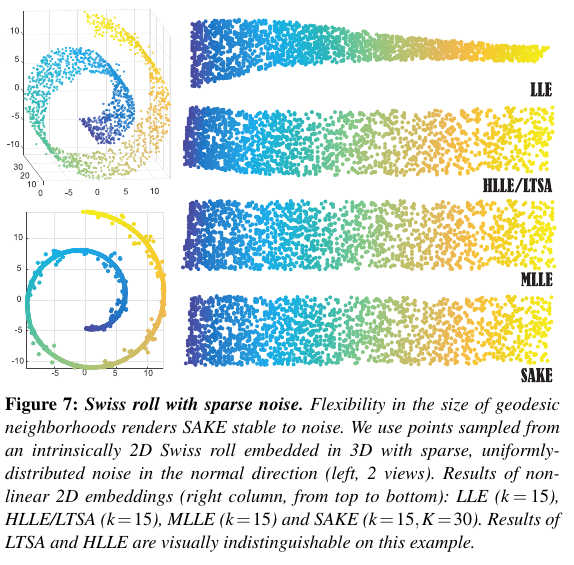
\includegraphics[width=0.8\textwidth]{img/sparse_noise}
      };
    }
    \visible<2> {
      \node at (0, 0) {
        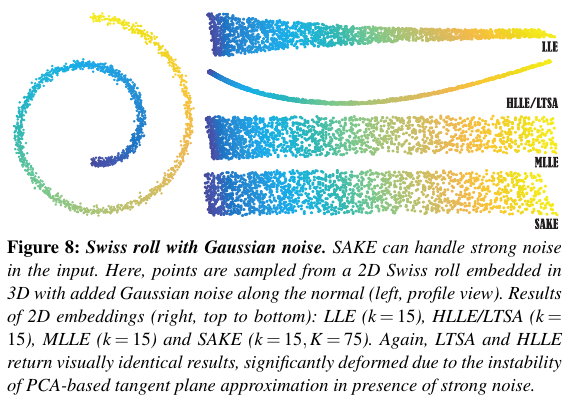
\includegraphics[width=0.8\textwidth]{img/gaussian_noise}
      };
    }
  }
\end{frame}

\begin{frame}
  \frametitle{Geodesic distance computation}
  \begin{itemize}
  \item For any pair $p, q$, the geodesic distance is approxiamted as
    the shortest path.
  \item Geodesic correction
    \begin{figure}
      \centering
      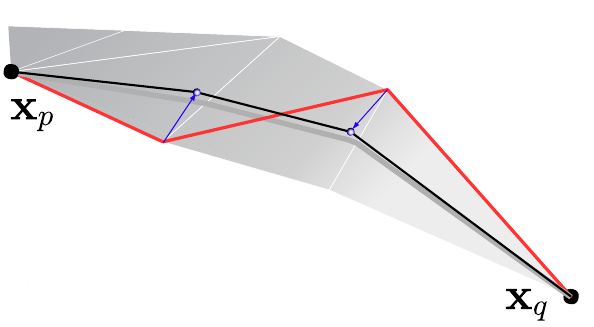
\includegraphics[width=0.6\textwidth]{img/geodesic_correction}       
    \end{figure}
  \end{itemize}
  \TikzDraw {
    \visible<2> {
      \node at (0, 0) {
        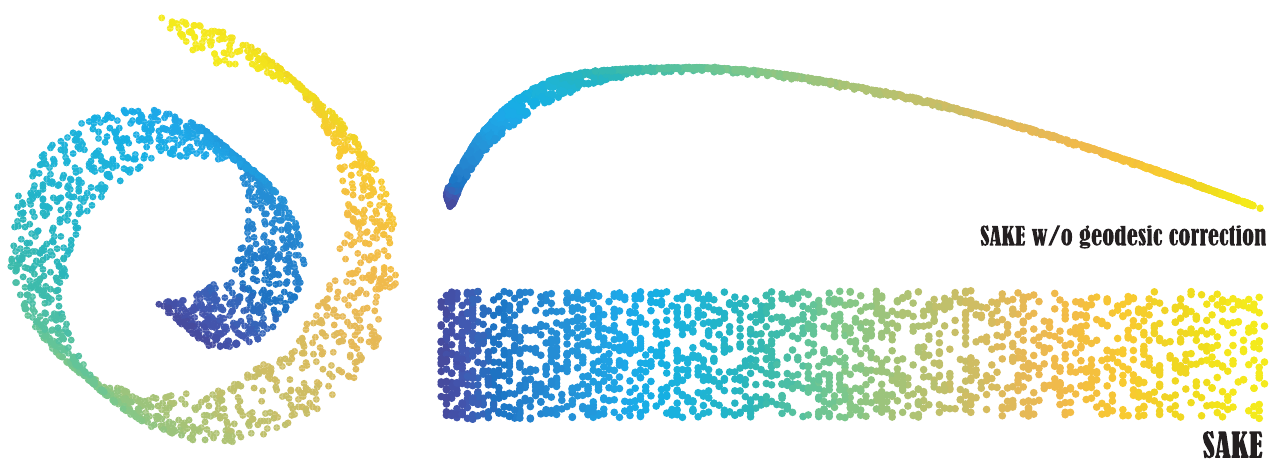
\includegraphics[width=\textwidth]{img/eval_geodesic_correction}
        };
    }
  }
\end{frame}

\begin{frame}
  \frametitle{Local embedding}
  \begin{itemize}
  \item Extract distance matrix
    \begin{equation*}
      D_i = (l_{pq})
    \end{equation*}
  \item Multidimensional scaling
    \begin{equation*}
     \argmin_Y \|YY^T-G_i\|_F^2, \text{~s.t.~~rank}(Y) = d.
    \end{equation*}
  \item Gram matrix through double centering
    \begin{equation*}
      \begin{split}
        &G_i = -\frac{HD^2H}{2} \\
        &H_{ij} = \delta_{ij}-1/N
      \end{split}
    \end{equation*}
  \end{itemize}
\end{frame}

\begin{frame}
  \frametitle{Assemble $L_i$}
  \begin{itemize}
  \item Embedded points
    \begin{equation*}
      Y_i = (y_i, y_{j_1}, \dots, y_{j_K})^T \in R^{(K+1)\times d}
    \end{equation*}
  \item Edge vector
    \begin{equation*}
      E_i = (y_{j_1}-y_i; \dots; y_{j_K}-y_i) \in R^{d\times K}
    \end{equation*}
  \item Find the kernel: $E_i = U\Lambda V^T$
  \item For one certain sigular vector $w^p \in R^K$
    \begin{equation*}
      E_i w^p = \sum_{j\in \mathcal{N}(i)} w^p_j(y_{j}-y_i) = 0
    \end{equation*}
  \end{itemize}
\end{frame}

\begin{frame}
  \frametitle{Assemble $L_i$}
  \begin{itemize}
  \item In matrix form $L_i \in R^{(K-d)\times (K+1)}$
    \begin{equation*}
      L_i = 
      \begin{pmatrix}
        \sum_m w^1_{j_m} & w^1_{j_1} & \dots & w^1_{j_K} \\
        \sum_m w^2_{j_m} & w^2_{j_1} & \dots & w^2_{j_K} \\
        \vdots & \vdots & \vdots &\vdots \\
        \sum_m w^{K-d}_{j_m} & w^{K-d}_{j_1} & \dots & w^{K-d}_{j_K} 
      \end{pmatrix}
    \end{equation*}
  \item Affine kernel
    \begin{equation*}
      L_i
      \begin{pmatrix}
        a^Ty_{i}+b \\
        a^Ty_{j_1}+b \\
        \vdots \\
        a^Ty_{j_K}+b         
      \end{pmatrix}
      =0
    \end{equation*}
  \end{itemize}
\end{frame}

\begin{frame}
  \frametitle{Extract final embedding}
  \begin{itemize}
  \item Global quadratic form
    \begin{equation*}
      Q = \sum_{i = 1}^n S_i^TL_i^TL_iS_i
    \end{equation*}
  \item Final embedding $Z \in R^{n\times d}$
    \begin{equation*}
      \argmin_Z \frac{1}{2}\text{tr}(Z^TQZ), \text{~~s.t.~~} Z^TZ = Id
    \end{equation*}
  \item Extract smallest $(d+1)$ eigenvectors
  \end{itemize}
\end{frame}

\begin{frame}
  \frametitle{Summary}
  \begin{itemize}
  \item \emph{\TODO{Preserve the local relative coordinates as best as possible.}}
  \item Exact recover for pointset sampled from a developable manifold
  \end{itemize}
\end{frame}

\begin{frame}
  \frametitle{Results}
  \begin{figure}
    \centering
    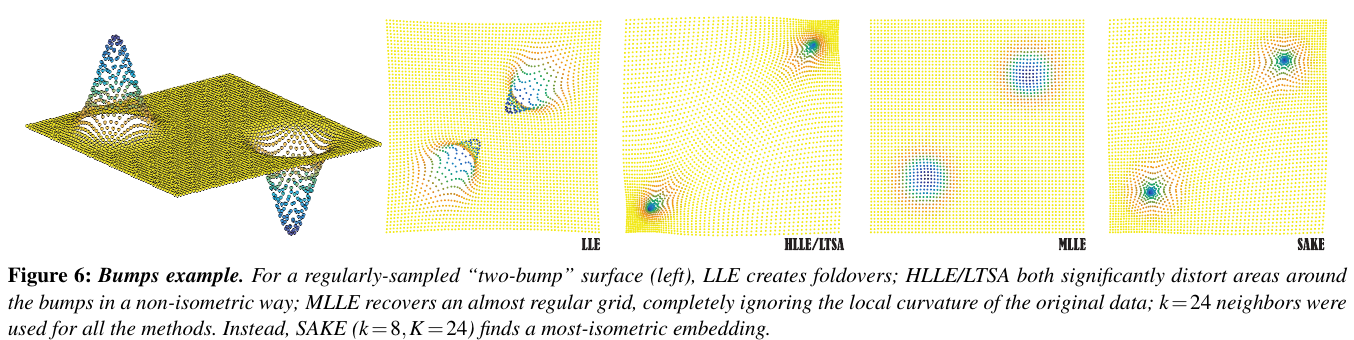
\includegraphics[width=\textwidth]{img/bumps}
  \end{figure}
\end{frame}

\begin{frame}
  \frametitle{Results}
  \begin{figure}
    \centering
    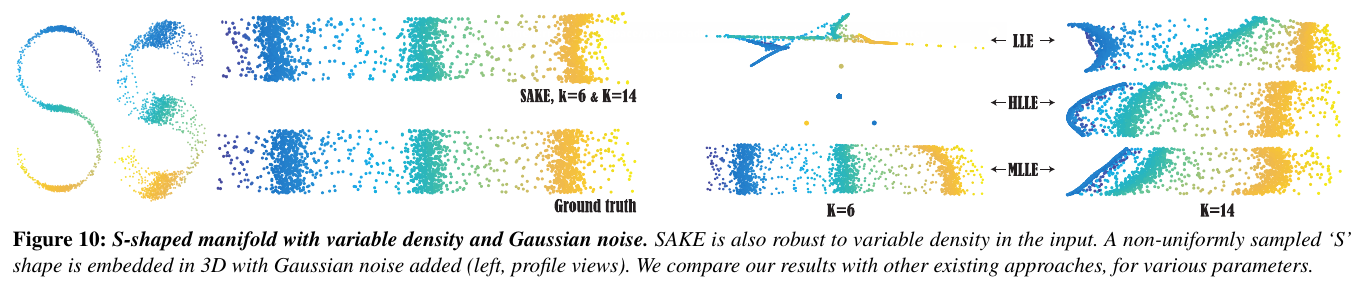
\includegraphics[width=\textwidth]{img/s_shape}
  \end{figure}
\end{frame}

\begin{frame}
  \frametitle{Results}
  \centering
  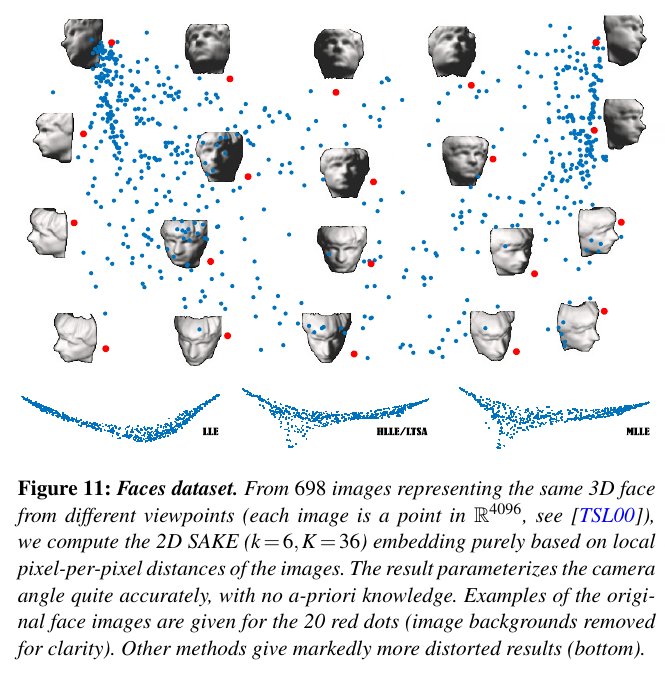
\includegraphics[width=0.7\textwidth]{img/faces_data}
\end{frame}

\begin{frame}
  \frametitle{Results}
  Deformation
  \begin{figure}
    \centering
    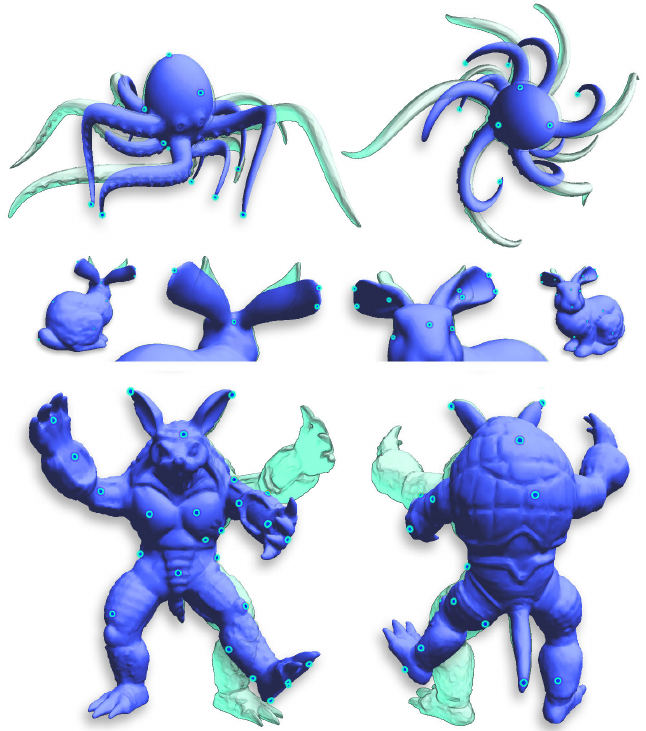
\includegraphics[width=0.6\textwidth]{img/sake_deformation}
  \end{figure}
\end{frame}

\begin{frame}
  \frametitle{Comments}
  \begin{itemize}
  \item Preconditioner?
  \item Generalize the concept of ``invariance of local coordinate''.
  \end{itemize}
\end{frame}

\begin{frame} 
  \TikzDraw {
    \node at (0, 0.5) {\Huge{Thanks!}};
  }
  %\gridlines
\end{frame}

\end{document}
